% Build from docs/: xelatex -jobname=Report Report.tex
\documentclass[conference,a4paper]{IEEEtran}
\usepackage{fontspec}
\setmainfont{Times New Roman}[SmallCapsFont=TeX Gyre Termes]
\setsansfont{Arial}
\setmonofont{Times New Roman}
\usepackage[vietnamese]{babel}
\usepackage{amsmath,amssymb,booktabs,array,graphicx,algorithmic,url,stfloats,balance}
\usepackage[hidelinks,unicode]{hyperref}
\graphicspath{{figures/benchmarks/}{figures/fashion/}{members/tv2/figures/}{members/tv3/}{members/tv3/figures/}}
\renewcommand{\figurename}{Hình}
\renewcommand{\tablename}{Bảng}
\renewcommand{\refname}{Tài liệu tham khảo}
\renewcommand{\algorithmicrequire}{\textbf{Đầu vào:}}
\renewcommand{\algorithmicensure}{\textbf{Đầu ra:}}
\newcommand{\bv}{\texttt{BitVector}}
\newcommand{\st}{\texttt{Set}}
\makeatletter
\newenvironment{reportfigure}{\par\medskip\noindent\begin{minipage}{\columnwidth}\def\@captype{figure}\centering}{\end{minipage}\par\medskip}
\newenvironment{reporttable}{\par\medskip\noindent\begin{minipage}{\columnwidth}\def\@captype{table}\centering}{\end{minipage}\par\medskip}
\makeatother
\begin{document}
\selectlanguage{vietnamese}
\renewcommand{\refname}{Tài liệu tham khảo}
\pagestyle{plain}
\title{Cài đặt và tối ưu Eclat bằng Julia\\cho phân tích giỏ hàng và khai thác mẫu trực quan}
\author{\IEEEauthorblockN{Nguyễn Thành Trung \qquad Lê Phúc Khang \qquad Nguyễn Võ Tấn Duy}
\IEEEauthorblockA{Đồ án môn Khai thác dữ liệu và ứng dụng\\Trường Đại học Khoa học Tự nhiên, ĐHQG-HCM}}
\maketitle
\begin{abstract}
Nhóm cài đặt thuật toán Eclat bằng Julia với hai cách biểu diễn tập
định danh giao dịch là Set và BitVector. Hai phiên bản trả về cùng
các tập phổ biến và số giao dịch hỗ trợ như SPMF trên năm bộ dữ liệu
đối chiếu. Phép đo trên bốn bộ dữ liệu cho thấy BitVector có đỉnh bộ
nhớ trung vị thấp hơn trên ba bộ, còn lợi thế về thời gian toàn tiến
trình thay đổi theo dữ liệu. Nhóm dùng cùng bộ khai thác để sinh luật
kết hợp từ giỏ hàng Groceries và tìm tổ hợp từ thị giác thường gặp
trong ảnh Fashion-MNIST. Hai ứng dụng minh họa cách lựa chọn biểu diễn
giao dịch và diễn giải các mẫu dựa trên dữ liệu quan sát.
\end{abstract}
\begin{IEEEkeywords}
Eclat, frequent itemset mining, Julia, BitVector, luật kết hợp, visual words.
\end{IEEEkeywords}
\section*{Mở đầu}
Cùng một nhóm sản phẩm có thể xuất hiện trong nhiều giỏ hàng,
và cùng một nhóm đặc trưng thị giác có thể xuất hiện trong nhiều
ảnh. Khi mỗi giỏ hoặc mỗi ảnh được biểu diễn dưới dạng giao dịch,
cả hai bài toán đều có thể dùng Eclat để tìm tổ hợp thường gặp.
Chương~I mô tả cách cài đặt và tối ưu thuật toán. Chương~II
đối chiếu kết quả với SPMF và khảo sát hiệu năng. Chương~III
trình bày cách tạo giao dịch và diễn giải các mẫu trong hai ứng dụng.

\section{Thuật toán Eclat và tối ưu hóa}
\label{sec:tv1}

\subsection{Bài toán và lựa chọn thuật toán}
Cho cơ sở dữ liệu giao dịch $D=(t_1,\ldots,t_N)$ trên tập mục $I$ có $M$ phần tử. Mỗi $t_j\subseteq I$ là một giao dịch. Hai giao dịch có nội dung giống nhau vẫn được tính riêng. Với tập mục $X\subseteq I$, \emph{support count} (số giao dịch chứa $X$) và \emph{relative support} (độ hỗ trợ tương đối) được định nghĩa:
\begin{equation}
 c(X)=|\{j:X\subseteq t_j\}|,\qquad s(X)=\frac{c(X)}{N}.
 \label{eq:tv1-support}
\end{equation}
Với $N>0$ và ngưỡng $s\in(0,1]$, bài toán \emph{frequent itemset mining} (khai thác tập phổ biến) yêu cầu tìm mọi $X\ne\varnothing$ thỏa $c(X)\ge c_{\min}$. Ngưỡng đếm tương ứng là
\begin{equation}
 c_{\min}=\lceil sN\rceil.
 \label{eq:tv1-threshold}
\end{equation}
Chẳng hạn, với $N=5$ và $s=0{,}5$, một tập cần xuất hiện trong ít nhất ba giao dịch.

Cài đặt sử dụng Eclat theo mô tả của Zaki~\cite{zaki}, với \emph{vertical representation} (biểu diễn dọc) và \emph{depth-first search}, DFS (duyệt theo chiều sâu). Apriori~\cite{agrawal} sinh ứng viên theo từng mức, còn Eclat tính số hỗ trợ bằng giao các tập định danh giao dịch. Cơ chế này cho phép khảo sát hai cấu trúc dữ liệu \texttt{Set} và \texttt{BitVector} trong Julia~\cite{julia} trên cùng quy trình duyệt. SPMF cung cấp cài đặt tham chiếu độc lập để kiểm chứng~\cite{spmf}.

\subsection{Biểu diễn dọc và nguyên tắc mở rộng}
Với mỗi $X$, đặt $T(X)=\{j:X\subseteq t_j\}$ là \emph{transaction-ID set}, TID-set (tập định danh giao dịch chứa $X$). Khi đó:
\begin{equation}
 T(X\cup Y)=T(X)\cap T(Y),\qquad c(X)=|T(X)|.
 \label{eq:tv1-intersection}
\end{equation}
Ví dụ, với $D=(\{1,2,3\},\{1,3\},\{2,3\},\{1,2\})$, ta có $T(\{1\})=\{1,2,4\}$ và $T(\{2\})=\{1,3,4\}$. Vì vậy $T(\{1,2\})=\{1,4\}$, nên số giao dịch hỗ trợ bằng 2. Nếu $s=0{,}5$, tập $\{1,2\}$ phổ biến nhưng $\{1,2,3\}$ không phổ biến vì chỉ xuất hiện một lần.

Các mục được sắp theo mã tăng dần. Tại tiền tố $P$, danh sách mở rộng chứa các cặp $(i,T(P\cup\{i\}))$. Những tập có chung tiền tố tạo thành một \emph{equivalence class} (lớp tương đương); mỗi nhánh chỉ ghép một mục với các mục đứng sau nó. Độ hỗ trợ có tính \emph{anti-monotonicity} (phản đơn điệu): nếu $X\subseteq Y$ thì $T(Y)\subseteq T(X)$, suy ra $c(Y)\le c(X)$. Do đó, khi một phép giao cho số hỗ trợ nhỏ hơn $c_{\min}$, toàn bộ nhánh mở rộng tương ứng được loại.

\subsection{Quy trình khai thác và tính đúng đắn}
Đầu tiên, thuật toán dựng TID-set của từng mục, giữ các tập một mục đạt $c_{\min}$ và sắp theo ID. Sau đó gọi thủ tục trong Bảng~\ref{tab:tv1-pseudocode} với tiền tố rỗng. TID-set của mỗi ứng viên đã bao gồm điều kiện xuất hiện của toàn bộ tiền tố, nên phép giao ở bước 7 tạo đúng TID-set cho tập mở rộng.

\begin{table}[t]
\caption{Giả mã DFS dùng chung cho hai phiên bản Eclat.}
\label{tab:tv1-pseudocode}
\begin{minipage}{\columnwidth}
\small
\begin{algorithmic}[1]
\REQUIRE Tiền tố $P$; danh sách $C=[(i,A_i)]$ tăng theo ID, với $A_i=T(P\cup\{i\})$, $|A_i|\ge c_{\min}$; ngưỡng $c_{\min}$.
\ENSURE Bổ sung mọi tập phổ biến thuộc nhánh $P$ vào $R$.
\FOR{mỗi vị trí $a$ trong $C$}
  \STATE $(i,A)\gets C[a]$; $Q\gets P\cup\{i\}$
  \STATE $R[Q]\gets |A|$
  \STATE $C'\gets [\,]$
  \FOR{mỗi vị trí $b>a$ trong $C$}
    \STATE $(j,B)\gets C[b]$
    \STATE $H\gets A\cap B$
    \IF{$|H|\ge c_{\min}$}
      \STATE Thêm $(j,H)$ vào $C'$
    \ENDIF
  \ENDFOR
  \IF{$C'\ne[\,]$}
    \STATE Gọi EclatDFS$(Q,C',c_{\min},R)$
  \ENDIF
\ENDFOR
\end{algorithmic}
\end{minipage}
\end{table}

\textit{Số hỗ trợ chính xác.} Ở gốc, mỗi TID-set được dựng trực tiếp từ giao dịch. Nếu các TID-set tại một mức là đúng, công thức~\eqref{eq:tv1-intersection} bảo đảm tập ở mức kế tiếp cũng đúng. Do đó mọi số hỗ trợ trả về đều bằng số giao dịch thực sự chứa tập mục.

\textit{Đầy đủ và không lặp.} Mỗi tập mục có duy nhất một thứ tự tăng dần. Nếu tập đó phổ biến, mọi tiền tố của nó cũng phổ biến theo tính phản đơn điệu, nên đường mở rộng tương ứng không bị cắt bỏ. Quy tắc chỉ ghép với mục đứng sau bảo đảm đường này được duyệt đúng một lần. Thuật toán vì vậy xuất toàn bộ tập phổ biến, mỗi tập xuất hiện đúng một lần.

\subsection{Cài đặt với Set và BitVector}
Phiên bản cơ sở dùng \texttt{Set} để lưu các định danh giao dịch chứa
từng mục. Phép giao xét các định danh thực sự có mặt, phù hợp khi một
mục chỉ xuất hiện trong ít giao dịch. Chi phí lưu trữ gồm các định danh
và cấu trúc bảng băm.

Phiên bản tối ưu dùng \texttt{BitVector} với $N$ bit. Bit thứ $j$ cho
biết giao dịch $j$ có chứa mục đang xét hay không. Phép AND theo bit
tạo giao, sau đó số bit bật cho biết số giao dịch hỗ trợ. Mỗi phép AND
có thể xử lý nhiều bit cùng lúc. Lợi thế này dễ thấy khi tập định danh
dày, còn với tập thưa, thuật toán vẫn phải quét các bit bằng 0.

Phiên bản tối ưu đếm số giao dịch chứa từng mục trước khi cấp phát
vector. Chỉ các tập một mục đạt ngưỡng mới cần vector bit. Cách làm
này thêm một lượt quét dữ liệu để giảm số vector phải lưu, đặc biệt
khi nhiều mục hiếm. Hai phiên bản dùng cùng quy tắc cắt nhánh và trả
về cùng loại kết quả. Vì phiên bản tối ưu thay đổi cả cách biểu diễn
lẫn bước cấp phát, chênh lệch trong thực nghiệm là tác động kết hợp
của hai thay đổi.

\subsection{Độ phức tạp và giới hạn}
Với \texttt{Set}, chi phí kỳ vọng của một phép giao tỷ lệ với kích
thước tập nhỏ hơn, giả sử tra cứu bảng băm có chi phí kỳ vọng hằng số.
Với \texttt{BitVector}, giao và đếm cần $O(\lceil N/w\rceil)$ thao tác
trên các từ máy, trong đó $w$ là số bit mỗi từ. Do đó, mật độ tập định
danh và số phép giao ảnh hưởng đến thời gian theo những cách khác nhau
ở hai phiên bản.

Số kết quả cũng ảnh hưởng đến cả thời gian và bộ nhớ. Với $M$ mục,
trường hợp xấu nhất có $2^M-1$ tập phổ biến khác rỗng. Ngay cả khi từng
phép giao nhanh, việc liệt kê và lưu toàn bộ tập phổ biến vẫn có thể
tốn nhiều tài nguyên.

\subsection{Đầu vào, đầu ra và kiểm chứng}
Cài đặt đọc giao dịch theo định dạng văn bản của SPMF. Mỗi mục chỉ
được tính một lần trong từng giao dịch, còn các giao dịch có nội dung
giống nhau được giữ riêng. Kết quả gồm các tập mục cùng số giao dịch
hỗ trợ. Công cụ dòng lệnh cho phép chọn ngưỡng hỗ trợ, cách biểu diễn
và đường dẫn tệp vào, tệp ra.

Nhóm dùng phép đếm vét cạn trên dữ liệu nhỏ để kiểm tra thuật toán
bằng một cách tính độc lập. Chương~II trình bày đối chiếu từng tập mục
và số hỗ trợ với SPMF trên năm bộ dữ liệu đầy đủ, sau đó khảo sát chi
phí của hai cách cài đặt khi thay đổi ngưỡng và đặc điểm giao dịch.

\section{Thực nghiệm và đánh giá}
\label{sec:benchmark}
\subsection{Câu hỏi thực nghiệm và phạm vi}
Thực nghiệm trước hết kiểm tra hai phiên bản Eclat bằng kết quả
tham chiếu từ SPMF. Sau đó, nhóm khảo sát thời gian chạy, đỉnh bộ nhớ
và ảnh hưởng của số lượng cũng như độ dài giao dịch. So sánh hiệu năng
dựa trên các lượt chạy hoàn tất và trả về kết quả đã đối chiếu.

\subsection{Dữ liệu và ngưỡng hỗ trợ}
Bốn bộ dữ liệu từ FIMI~\cite{fimi} có đặc điểm khác nhau
(Bảng~\ref{tab:data}). Chess và Mushroom có giao dịch dài. Retail
có nhiều mục nhưng mỗi giao dịch thường ngắn. T10I4D100K là dữ liệu
tổng hợp. Số tập phổ biến phụ thuộc vào mức độ đồng xuất hiện của
các mục và ngưỡng hỗ trợ, ngoài quy mô của bộ dữ liệu.

\begin{reporttable}
\caption{Số giao dịch $N$, số mục phân biệt $M$ và độ dài giao dịch trung bình $\bar L$ sau chuẩn hóa.}
\label{tab:data}
\small
\begin{tabular}{lrrr}\toprule
Bộ dữ liệu & $N$ & $M$ & $\bar L$\\\midrule
Chess & 3.196 & 75 & 37,0000\\
Mushroom & 8.124 & 119 & 23,0000\\
Retail & 88.162 & 16.470 & 10,3058\\
T10I4D100K & 100.000 & 870 & 10,1023\\\bottomrule
\end{tabular}
\end{reporttable}

Julia và SPMF nhận cùng dữ liệu sau khi chuẩn hóa. Bước này giữ
nguyên các giao dịch trùng và dùng ánh xạ một-một nếu cần đổi mã mục.
Với mỗi bộ dữ liệu, nhóm chọn bảy mức của ngưỡng hỗ trợ tối thiểu
(\textit{minsup}) rồi áp dụng công thức~\eqref{eq:tv1-threshold}.
Các giá trị cụ thể được liệt kê ở Bảng~\ref{tab:grids} trong phụ lục.

\subsection{Môi trường và phương pháp đo}
\label{sec:measurement-method}
Các phép đo chạy trên cùng môi trường Colab CPU (Broadwell, 2 vCPU,
12,67 GiB RAM). Cài đặt Julia dùng phiên bản 1.13.3 và một luồng.
Mỗi cấu hình có năm lượt đo. Các hình báo cáo trung vị và khoảng
nhỏ nhất đến lớn nhất để thể hiện độ biến thiên giữa các lượt.

\textit{Thời gian toàn tiến trình.} Mỗi lượt dùng một tiến trình
mới, tính từ khi khởi động đến khi ghi xong kết quả. Khoảng đo bao
gồm nạp môi trường, biên dịch JIT, đọc dữ liệu, dựng tập định danh
và khai thác. Chuẩn hóa dữ liệu và đối chiếu kết quả được thực hiện
ngoài khoảng đo này.

\textit{Thời gian khai thác sau làm nóng.} Thí nghiệm về quy mô và
độ dài giao dịch đo lời gọi khai thác sau một lượt chạy chuẩn bị
(\textit{warm-up}) với cùng dữ liệu và ngưỡng.

\textit{Đỉnh bộ nhớ thường trú (Peak RSS).} Đây là giá trị lớn nhất
của bộ nhớ thường trú từ lúc tiến trình khởi động đến khi khai thác
xong, trước khi sắp xếp và ghi kết quả. Giá trị này gồm cả môi trường
Julia, lượt chạy chuẩn bị, dữ liệu đầu vào và các cấu trúc khai thác.

\subsection{Đối chiếu tính đúng đắn}
Một lần đối chiếu đạt khi cài đặt của nhóm và SPMF trả về đúng cùng
các tập mục và cùng số giao dịch hỗ trợ cho từng tập. Hai kết quả
có cùng số lượng vẫn có thể khác nhau ở các tập mục cụ thể. Bảng~\ref{tab:correct}
trình bày kết quả đối chiếu trên năm bộ dữ liệu đầy đủ.

\begin{reporttable}
\caption{Kết quả đối chiếu từng tập mục và số hỗ trợ với SPMF.}
\label{tab:correct}
\footnotesize
\begin{tabular}{lrrr}\toprule
Bộ dữ liệu & Ngưỡng (\%) & Số tập SPMF & Khớp\\\midrule
Groceries & 1 & 333 & 100\%\\
Chess & 87,5 & 1.386 & 100\%\\
Mushroom & 70 & 31 & 100\%\\
Retail & 4 & 18 & 100\%\\
T10I4D100K & 1,5 & 237 & 100\%\\\bottomrule
\end{tabular}
\end{reporttable}

\subsection{Thời gian chạy và số tập mục theo ngưỡng}
Nhóm chạy Set, BitVector và SPMF ở bảy ngưỡng trên mỗi bộ dữ liệu.
Bảng~\ref{tab:runtime-colab} tóm tắt kết quả ở ngưỡng thấp nhất
của từng bộ. Hình~\ref{fig:runtime-colab} so sánh xu hướng trên cả dải.

\begin{reporttable}
\caption{Thời gian toàn tiến trình ở ngưỡng thấp nhất (giây). Trung vị của năm lượt trên Colab. BV là BitVector.}
\label{tab:runtime-colab}
\footnotesize
\begin{tabular}{lrrrrr}\toprule
Bộ dữ liệu & $s$ (\%) & Set & BV & SPMF & Số tập\\\midrule
Chess & 80 & 6,365 & 6,286 & 2,156 & 8.227\\
Mushroom & 40 & 3,890 & 5,147 & 1,235 & 565\\
Retail & 0,5 & 4,617 & 5,052 & 2,598 & 580\\
T10I4D100K & 0,5 & 10,855 & 5,422 & 1,774 & 1.073\\\bottomrule
\end{tabular}
\end{reporttable}

\begin{figure*}[!tbp]
\centering
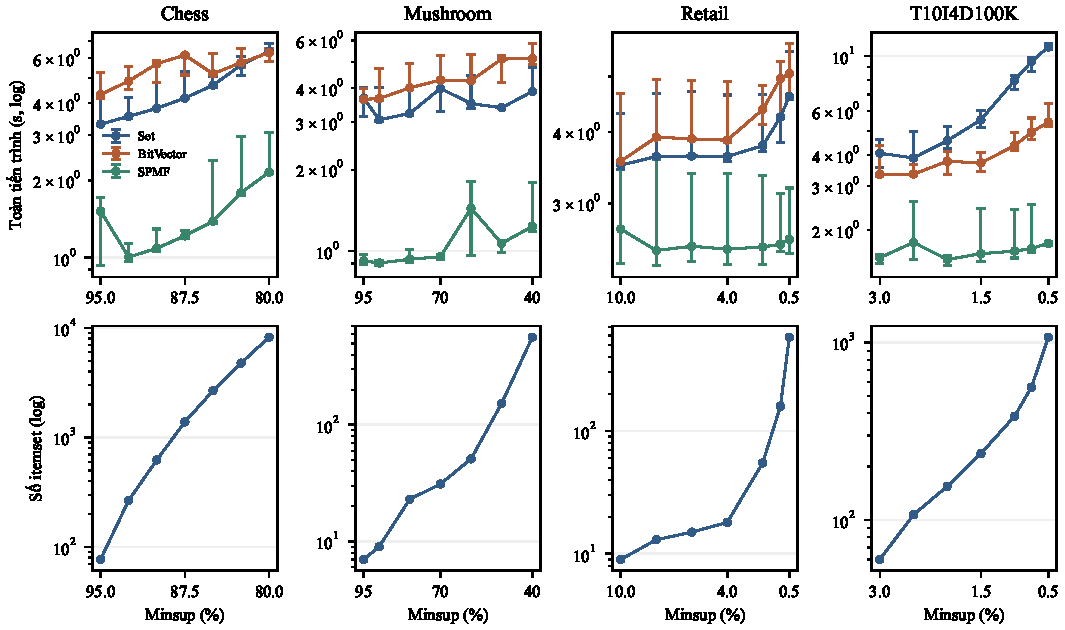
\includegraphics[width=0.90\textwidth]{runtime_counts.pdf}
\caption{Thời gian toàn tiến trình (hàng trên) và số tập phổ biến (hàng dưới) trên bốn bộ dữ liệu theo ngưỡng hỗ trợ giảm dần. Điểm biểu thị trung vị, thanh biểu thị khoảng nhỏ nhất đến lớn nhất. Trục tung dùng thang logarit.}
\label{fig:runtime-colab}
\end{figure*}



SPMF có thời gian toàn tiến trình thấp nhất theo trung vị ở cả
28 cấu hình. Trong hai phiên bản của nhóm, BitVector nhanh hơn
trên T10I4D100K, còn Set nhanh hơn trên Retail ở cả bảy ngưỡng.
Retail có trung bình khoảng 10 mục mỗi giao dịch trên tổng số hơn
16 nghìn mục, nên cách biểu diễn chỉ lưu các định danh xuất hiện
có thể có lợi. Trên Chess ở ngưỡng 80\%, hai
phiên bản chỉ chênh khoảng 1,2\% và khoảng thời gian quan sát
được chồng lấn.

Khi hạ ngưỡng, các tập đã phổ biến được giữ lại và các tập có
số hỗ trợ thấp hơn có thể được bổ sung. Chess có ít giao dịch
nhất nhưng cho nhiều kết quả nhất ở cuối dải khảo sát. Các bộ
dữ liệu dùng các dải ngưỡng khác nhau, nên kết quả này mô tả
xu hướng trong từng dải đã chọn.

\subsubsection{Đối chiếu hiệu năng với SPMF}
Ở ngưỡng thấp nhất của T10I4D100K, thời gian toàn tiến trình của Set
và BitVector lần lượt gấp khoảng 6,12 và 3,06 lần SPMF
(Bảng~\ref{tab:runtime-colab}). Thay biểu diễn Set bằng vector bit
thu hẹp chênh lệch trong cấu hình này, nhưng SPMF vẫn có lợi thế
về thời gian hoàn tất. Trên Mushroom và Retail ở cuối dải ngưỡng,
Set lại gần thời gian của SPMF hơn BitVector. Kết quả vì vậy chưa
ủng hộ việc dùng một biểu diễn duy nhất cho mọi bộ dữ liệu.

Phép đo toàn tiến trình ở Mục~\ref{sec:measurement-method} phản ánh
chi phí của một lượt chạy độc lập. Julia phải nạp môi trường và
biên dịch các lời gọi chưa được thực thi; SPMF cũng chịu chi phí
khởi động JVM, đọc ghi và thực thi Java. Do chưa đo tách công đoạn
hoặc đo khai thác sau làm nóng của SPMF, chưa thể quy chênh lệch
cho riêng ngôn ngữ, phép giao TID-set hay tối ưu nội bộ của SPMF.
So sánh Peak RSS
chỉ gồm Set và BitVector, nên chưa cho phép đối chiếu RAM với SPMF.

\subsection{Đỉnh bộ nhớ ở ngưỡng giữa dải}
Nhóm dùng ngưỡng thứ tư của mỗi bộ dữ liệu. Mỗi lượt đo chạy một
phiên bản trong tiến trình riêng. Bảng~\ref{tab:ram-colab} và
Hình~\ref{fig:ram-colab} tổng hợp trung vị của năm lượt.

\begin{reporttable}
\caption{Peak RSS trung vị (MiB), năm tiến trình cho mỗi phiên bản. $\Delta_M$ là mức giảm từ trung vị của Set sang BV.}
\label{tab:ram-colab}
\small
\begin{tabular}{lrrr}\toprule
Bộ dữ liệu & Set & BV & $\Delta_M$ (\%)\\\midrule
Chess & 385,27 & 374,90 & 2,69\\
Mushroom & 374,90 & 374,90 & 0,00\\
Retail & 444,45 & 378,34 & 14,87\\
T10I4D100K & 437,32 & 418,77 & 4,24\\\bottomrule
\end{tabular}
\end{reporttable}

\begin{figure}[!tbp]
\centering
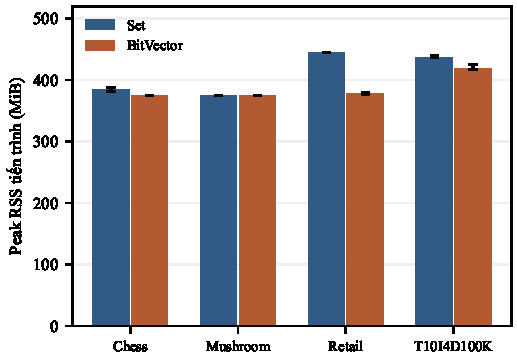
\includegraphics[width=\columnwidth]{peak_ram.pdf}
\caption{Đỉnh bộ nhớ ở ngưỡng giữa dải. Cột biểu thị trung vị và thanh dọc biểu thị khoảng nhỏ nhất đến lớn nhất. Đỉnh gồm cả môi trường Julia và dữ liệu đầu vào.}
\label{fig:ram-colab}
\end{figure}

BitVector có đỉnh bộ nhớ trung vị thấp hơn trên ba bộ dữ liệu,
với mức giảm rõ nhất trên Retail (14,87\%). Với Retail, 7 trên
16.470 mục đạt ngưỡng 4\%, nên việc cấp vector sau khi lọc đặc
biệt có ích. Trên Mushroom, hai trung vị bằng nhau. Đây là mức dùng
bộ nhớ của cả tiến trình theo phạm vi ở Mục~\ref{sec:measurement-method}.

\subsection{Khả năng mở rộng theo số giao dịch}
Nhóm tạo năm tập con lồng nhau từ Retail ở các mức 10\%, 25\%,
50\%, 75\% và 100\%. Ngưỡng hỗ trợ giữ ở 4\%, nên số giao dịch
tối thiểu thay đổi theo kích thước mỗi tập con. Bảng~\ref{tab:scale-colab}
và Hình~\ref{fig:scale-colab} trình bày thời gian khai thác sau làm nóng.

\begin{reporttable}
\caption{Khả năng mở rộng trên Retail: trung vị thời gian khai thác sau làm nóng (ms), năm lượt/cấu hình.}
\label{tab:scale-colab}
\footnotesize
\begin{tabular}{rrrrr}\toprule
Tỷ lệ (\%) & $N$ & $c_{\min}$ & Set & BV\\\midrule
10 & 8.816 & 353 & 25,08 & 6,10\\
25 & 22.040 & 882 & 68,92 & 16,71\\
50 & 44.081 & 1.764 & 158,70 & 33,80\\
75 & 66.121 & 2.645 & 276,07 & 49,34\\
100 & 88.162 & 3.527 & 358,41 & 62,95\\\bottomrule
\end{tabular}
\end{reporttable}

\begin{figure}[!tbp]
\centering
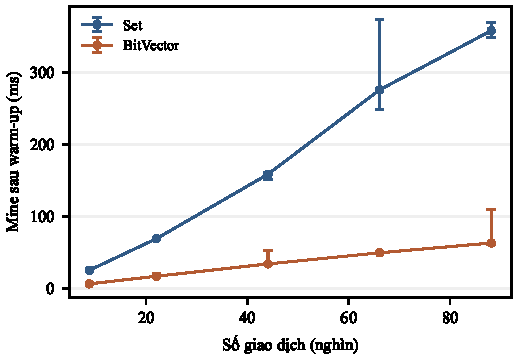
\includegraphics[width=\columnwidth]{scalability.pdf}
\caption{Khả năng mở rộng trên năm tập con lồng nhau của Retail. Điểm biểu thị trung vị và thanh biểu thị khoảng nhỏ nhất đến lớn nhất. Hai phiên bản khớp SPMF ở mọi mức.}
\label{fig:scale-colab}
\end{figure}

Hình~\ref{fig:scale-colab} cho thấy khi $N$ tăng khoảng mười lần,
trung vị của Set tăng 14,29 lần, còn BitVector tăng 10,32 lần. Cả năm mức đều
có 18 tập mục, nên số kết quả giữ nguyên trong thí nghiệm này. BitVector
có xu hướng tăng gần tỷ lệ với $N$ trong miền đã đo. Thời gian của Set tăng nhanh hơn.
Xu hướng này chỉ mô tả các tập con Retail và ngưỡng đã khảo sát.

\subsection{Phân tích đánh đổi giữa thời gian và bộ nhớ}
Trên Retail tại ngưỡng hỗ trợ 4\%, BitVector có Peak RSS trung vị
378,34 MiB, giảm 14,87\% so với mức 444,45 MiB của Set.
Thời gian toàn tiến trình của BitVector là 3,869 giây, cao hơn
mức 3,624 giây của Set, theo số đo đầy đủ của Hình~\ref{fig:runtime-colab}.
Trong thí nghiệm mở rộng theo số giao dịch,
trên toàn bộ 88.162 giao dịch và cùng ngưỡng hỗ trợ, thời gian
khai thác sau làm nóng lần lượt là 62,95 ms và 358,41 ms.

Sự khác biệt trong cách dựng biểu diễn dọc giúp giải thích xu hướng
bộ nhớ. Phiên bản Set dựng tập định danh giao dịch cho toàn bộ
16.470 mục rồi mới lọc các mục không đạt ngưỡng. Phiên bản BitVector
đếm số hỗ trợ trước và chỉ cấp vector cho 7 mục đạt ngưỡng 4\%.
Với $N$ giao dịch và $F_1$ mục đạt ngưỡng, các vector ban đầu cần
$O(F_1N)$ bit, bên cạnh trạng thái đếm $O(M)$ cho $M$ mục phân biệt.
Lọc trước cấp phát giảm số cấu trúc phải dựng khi có nhiều mục hiếm.
Do Peak RSS đo toàn tiến trình và hai phiên bản đồng thời thay đổi
cấu trúc lưu trữ lẫn quy trình cấp phát, chưa thể tách đóng góp
của từng yếu tố vào mức giảm bộ nhớ.

Phép đo sau làm nóng bao gồm cả dựng biểu diễn dọc và duyệt các nhánh
Eclat. Trên Retail ở ngưỡng đang xét, kết quả chỉ có 18 tập phổ biến.
Chênh lệch thời gian vì vậy cần được xem xét cùng chi phí lọc trước
cấp phát đã nêu ở trên. Các phép giao theo từ máy
cũng có thể đóng góp vào lợi thế của BitVector, nhưng chưa đủ cơ sở
quy toàn bộ chênh lệch cho thao tác này khi hai công đoạn chưa được đo riêng.

Hai phiên bản dùng chung mã đọc ghi và trả về cùng kết quả. Tuy vậy,
chưa có số đo từng công đoạn để giải thích chênh lệch 0,245 giây của
thời gian toàn tiến trình. Chỉ số này phù hợp với lượt chạy độc lập;
thời gian sau làm nóng phù hợp với khai thác khi mã đã được biên dịch.
Lựa chọn phiên bản cần xét cả bối cảnh chạy và giới hạn RAM.

\subsection{Ảnh hưởng của độ dài giao dịch}
Nhóm tạo 5.000 giao dịch từ 64 mục và tăng độ dài mỗi giao dịch
từ 4 lên 20, với năm mức khảo sát. Số giao dịch, số mục có thể
chọn và ngưỡng hỗ trợ 5\% được giữ cố định. Bảng~\ref{tab:length-colab}
và Hình~\ref{fig:length-colab} cho thấy thời gian cùng số tập phổ
biến ở từng mức.

\begin{reporttable}
\caption{Dữ liệu tổng hợp và trung vị thời gian khai thác sau làm nóng (ms), qua năm lượt mỗi cấu hình.}
\label{tab:length-colab}
\footnotesize
\begin{tabular}{rrrrr}\toprule
$L$ & Mật độ (\%) & Số tập & Set & BV\\\midrule
4 & 6,25 & 64 & 23,81 & 1,40\\
8 & 12,50 & 64 & 51,29 & 2,39\\
12 & 18,75 & 64 & 85,16 & 3,14\\
16 & 25,00 & 2.077 & 691,57 & 10,18\\
20 & 31,25 & 2.080 & 1.055,70 & 11,10\\\bottomrule
\end{tabular}
\end{reporttable}

\begin{figure*}[!tbp]
\centering
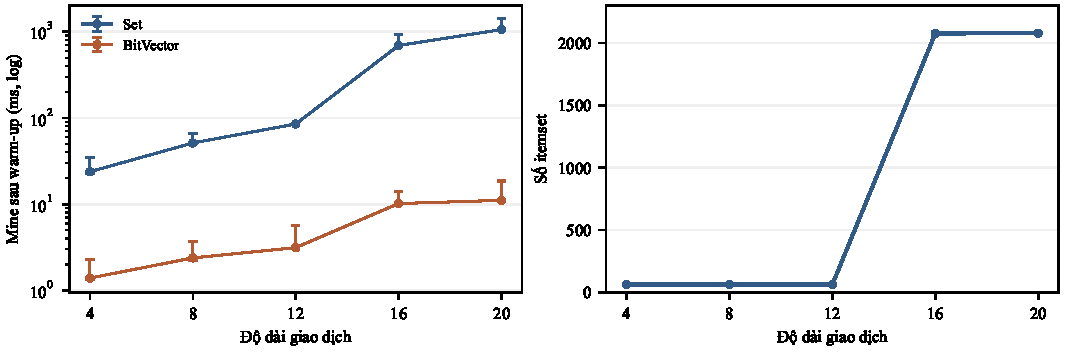
\includegraphics[width=\textwidth]{transaction_length.pdf}
\caption{Ảnh hưởng độ dài giỏ với $N=5.000$, $M=64$, ngưỡng hỗ trợ cố định ở 5\%. Trái: trung vị và khoảng biến thiên của thời gian khai thác trên trục tung log. Phải: số tập mục khớp SPMF ở cả hai phiên bản.}
\label{fig:length-colab}
\end{figure*}

Bước tăng từ 12 lên 16 mục mỗi giao dịch làm số kết quả tăng từ
64 lên 2.077. Giỏ dài hơn làm tăng khả năng hai mục xuất hiện cùng
nhau, nên nhiều cặp vượt ngưỡng 250 giao dịch. Eclat vì thế giữ thêm
các nhánh mở rộng và thực hiện nhiều công việc hơn. Khi độ dài tăng
tiếp lên 20 mục, số kết quả gần như giữ nguyên nhưng thời gian của
Set vẫn tăng đáng kể. Số tập được trả về vì vậy chỉ giải thích một
phần chi phí khai thác.

Với $N$ giữ cố định, chi phí quét một vector bit cho mỗi phép giao
vẫn tỷ lệ với $\lceil N/w\rceil$, trong đó $w$ là số bit mỗi từ máy.
Ở Set, chi phí giao kỳ vọng tỷ lệ với tập định danh nhỏ hơn; khi
giỏ dài lên, nhiều mục có mặt trong nhiều giao dịch hơn, làm tăng
khối lượng định danh cần xử lý. Cơ chế này phù hợp với việc thời gian
Set tiếp tục tăng khi $L$ từ 16 lên 20 dù số kết quả gần như không đổi.
Tuy nhiên, thực nghiệm chưa ghi số ứng viên và kích thước từng tập
định danh, nên chưa xác định riêng phần thời gian tăng do giao tập,
dựng biểu diễn hay cấp phát tạm.

\subsection{Thảo luận và giới hạn thực nghiệm}
Cả 560 lượt đo đều hoàn tất và cho kết quả khớp với SPMF. Lợi thế về
thời gian của mỗi phiên bản phụ thuộc vào độ thưa của tập định danh,
dải ngưỡng và phạm vi đo. Xu hướng quan sát được trên một môi trường
Colab, với năm lượt cho mỗi cấu hình, cần được kiểm tra trên các môi
trường và bộ dữ liệu khác trước khi khái quát.

Có hai hướng tối ưu tiếp theo. Thứ nhất, có thể chọn cấu trúc thưa
hay vector bit theo mật độ của từng tập định danh và đo cả chi phí
chuyển đổi. Thứ hai, có thể dùng lại bộ đệm trong quá trình duyệt
theo chiều sâu để giảm cấp phát khi tính giao. Thí nghiệm tách
riêng từng thay đổi sẽ cho biết phần đóng góp của mỗi kỹ thuật.

\section{Ứng dụng thực tế}\label{sec:applications}
\subsection{Groceries: phân tích giỏ hàng}\label{sec:groceries}
\subsubsection{Bài toán và chuyển đổi dữ liệu}
Phân tích giỏ hàng (\textit{market basket analysis}) tìm các nhóm
sản phẩm thường được mua cùng nhau để sinh luật kết hợp~\cite{agrawal}.
Bộ dữ liệu Groceries~\cite{groceries} gồm 9.835 giỏ và 169 sản phẩm.
Nhóm chuẩn hóa tên, gán mã cho từng sản phẩm và xem mỗi giỏ là
một giao dịch. Sản phẩm lặp trong cùng giỏ chỉ được tính một lần.
Các giỏ giống nhau vẫn là những giao dịch riêng.

\subsubsection{Sinh luật và lựa chọn ngưỡng}
Từ một tập phổ biến $Z$ có ít nhất hai sản phẩm, nhóm chia $Z$
thành hai vế khác rỗng $X$ và $Y$ để lập luật $X\Rightarrow Y$.
Gọi $c(A)$ là số giỏ chứa toàn bộ tập $A$ và $N=9.835$ là tổng số giỏ.
\begin{align}
\operatorname{supp}(X\Rightarrow Y)&=\frac{c(X\cup Y)}{N},\\
\operatorname{conf}(X\Rightarrow Y)&=\frac{c(X\cup Y)}{c(X)},\\
\operatorname{lift}(X\Rightarrow Y)&=\frac{\operatorname{conf}(X\Rightarrow Y)}{c(Y)/N}.
\end{align}
Độ hỗ trợ (\textit{support}) cho biết tỷ lệ giỏ chứa cả hai vế.
Độ tin cậy (\textit{confidence}) là tỷ lệ giỏ có $Y$ trong số các
giỏ đã có $X$. Lift so tỷ lệ này với tần suất chung của $Y$.

Nhóm khảo sát bốn ngưỡng hỗ trợ tối thiểu (\textit{minsup}) và ba
ngưỡng tin cậy tối thiểu (\textit{minconf}), như trình bày trong
Bảng~\ref{tab:params}.

\begin{reporttable}
\caption{Số tập phổ biến và số luật theo các ngưỡng hỗ trợ và tin cậy. Ba cột cuối là số luật tại từng minconf.}\label{tab:params}
\centering\footnotesize
\begin{tabular}{rrrrr}\toprule
Hỗ trợ (\%) & Số tập & 30\% & 50\% & 70\% \\\midrule
0,5 & 1.001 & 487 & 120 & 1 \\
1,0 & 333 & 125 & 15 & 0 \\
2,0 & 122 & 37 & 1 & 0 \\
3,0 & 63 & 14 & 0 & 0 \\
\bottomrule\end{tabular}
\end{reporttable}

Khi tăng minsup từ 0,5\% lên 1\%, số tập
phổ biến giảm từ 1.001 xuống 333. Tại minconf 50\%, số luật tương ứng
giảm từ 120 xuống 15; nếu tăng minsup lên 2\% và 3\%, chỉ còn một luật
và không còn luật nào. Với 9.835 giao dịch, minsup 0,5\% và 1\%
tương ứng ít nhất 50 và 99 giỏ chứa đồng thời cả hai vế.
Nhóm chọn minsup 1\% để giữ mức hỗ trợ này và vẫn có đủ luật cho
bảng mười luật hàng đầu tại minconf 50\%. Nếu giảm minconf xuống 30\%, hai mức minsup 2\%
và 3\% vẫn cho 37 và 14 luật.

Tại minsup 1\%, tăng minconf từ 30\% lên 50\% thu hẹp tập luật
từ 125 xuống 15, còn mức 70\% loại toàn bộ luật. Ngưỡng 50\% yêu cầu
ít nhất một nửa số giỏ chứa vế trái cũng chứa vế phải trên dữ liệu
quan sát. Cấu hình 1\%/50\% giữ được một tập luật đủ gọn để đối chiếu
và diễn giải, so với 487 luật ở cấu hình 0,5\%/30\%.

Ngưỡng hỗ trợ 1\% bỏ qua các tổ hợp xuất hiện trong 50--98 giỏ
mà mức 0,5\% có thể giữ lại. Tăng minconf cũng có thể loại các luật
có lift cao nhưng độ tin cậy chưa đạt ngưỡng.
Nhóm xếp luật theo lift; các luật cùng lift
được phân hạng tiếp theo bằng độ tin cậy và độ hỗ trợ.

\subsubsection{Mười luật nổi bật và ý nghĩa kinh doanh}
Bảng~\ref{tab:rules} trình bày mười luật có lift cao nhất, sử dụng tên
sản phẩm gốc trong dữ liệu. Các luật 1--4 có vế phải là
\textit{other vegetables}, còn các luật 5--10 hướng tới
\textit{whole milk}. Các tổ hợp gồm cả hai vế có độ hỗ trợ
khoảng 1,01--1,45\%.

\begin{table*}[!t]
\caption{Mười luật Groceries có lift cao nhất ở ngưỡng hỗ trợ 1\% và độ tin cậy 50\%. Cột số giỏ đếm giao dịch chứa cả hai vế.}\label{tab:rules}
\centering\footnotesize
\begin{tabular}{rp{.31\textwidth}p{.15\textwidth}rrrr}\toprule
\# & Vế trái $X$ & Vế phải $Y$ & Số giỏ & Hỗ trợ (\%) & Tin cậy (\%) & Lift \\\midrule
1 & citrus fruit + root vegetables & other vegetables & 102 & 1,037 & 58,62 & 3,030 \\
2 & root vegetables + tropical fruit & other vegetables & 121 & 1,230 & 58,45 & 3,021 \\
3 & rolls/buns + root vegetables & other vegetables & 120 & 1,220 & 50,21 & 2,595 \\
4 & root vegetables + yogurt & other vegetables & 127 & 1,291 & 50,00 & 2,584 \\
5 & curd + yogurt & whole milk & 99 & 1,007 & 58,24 & 2,279 \\
6 & butter + other vegetables & whole milk & 113 & 1,149 & 57,36 & 2,245 \\
7 & root vegetables + tropical fruit & whole milk & 118 & 1,200 & 57,00 & 2,231 \\
8 & root vegetables + yogurt & whole milk & 143 & 1,454 & 56,30 & 2,203 \\
9 & domestic eggs + other vegetables & whole milk & 121 & 1,230 & 55,25 & 2,162 \\
10 & whipped/sour cream + yogurt & whole milk & 107 & 1,088 & 52,45 & 2,053 \\
\bottomrule\end{tabular}
\end{table*}

Nhóm luật 1--4 gợi ý khảo sát việc kết hợp các mặt hàng rau củ với
những giỏ đã có trái cây, bánh mì hoặc \textit{yogurt}. Chẳng hạn, luật số 1
được hỗ trợ bởi 102 trong 174 giỏ chứa đồng thời \textit{citrus fruit}
và \textit{root vegetables}, tương ứng độ tin cậy 58,62\%.
Trong toàn bộ dữ liệu, \textit{other vegetables} xuất hiện ở
1.903 giỏ, chiếm 19,35\%. Lift 3,030 cho biết tỷ lệ xuất hiện của
nhóm rau này trong các giỏ có vế trái cao hơn khoảng ba lần tỷ lệ
chung. Có thể thử nghiệm gợi ý nhóm rau này cho giỏ đã có vế trái.
Nhãn
\textit{other vegetables} vẫn là một nhóm rộng, nên dữ liệu chưa
cho biết loại rau cụ thể nào phù hợp để gợi ý.

Nhóm luật 5--10 đều có vế phải là \textit{whole milk}. Sản phẩm này
vốn phổ biến, xuất hiện trong 2.513 giỏ, tương ứng 25,55\% dữ liệu.
Vì vậy, độ tin cậy cần được đọc cùng lift để xét mức đồng xuất hiện
so với tần suất nền. Ở luật số 5, 99 trong 170 giỏ có
\textit{curd} và \textit{yogurt} cũng chứa \textit{whole milk}:
Độ tin cậy đạt 58,24\%, cao gấp 2,279 lần tỷ lệ chung của sữa.
Các luật về bơ, trứng và sản phẩm sữa có thể cung cấp nhóm ứng viên
cho gợi ý mua kèm hoặc bố trí trưng bày. Chúng chưa đủ để kết luận
người mua đang chuẩn bị cùng một món ăn hay có cùng nhu cầu sử dụng.

Trong một ứng dụng gợi ý, có thể kiểm tra các luật mà giỏ hiện tại
đã chứa vế trái và chưa chứa vế phải, rồi chọn sản phẩm để hiển thị.
Hai luật cùng vế trái \textit{root vegetables + tropical fruit}
nhưng khác vế phải ở hàng 2 và 7 cho thấy cần xử lý nhiều gợi ý
cùng lúc. Lift hỗ trợ xếp hạng liên hệ, còn số giỏ hỗ trợ cho biết
số lần tổ hợp đã được quan sát; dữ liệu hiện có chưa phản ánh
tồn kho, giá bán hoặc lợi nhuận để lựa chọn gợi ý theo hiệu quả kinh doanh.

\subsubsection{Kiểm chứng và thời gian thực thi}
Ở ngưỡng hỗ trợ 1\%, cả 333 tập mục và số hỗ trợ tương ứng đều khớp
với SPMF. Trên Colab CPU, toàn bộ quy trình từ đọc dữ liệu đến
sinh luật có thời gian trung vị 82,62 ms qua năm lượt sau làm nóng,
với phiên bản Set. Số đo theo từng công đoạn được lưu cùng kết quả thực nghiệm.

\subsubsection{Giới hạn áp dụng}
Luật mô tả đồng xuất hiện trong giỏ hoàn tất, không cho biết thứ tự mua
hoặc quan hệ nhân quả. Dữ liệu không có mã khách, thời gian, giá và khuyến
mãi. Mười luật và các ngưỡng được chọn trên cùng bộ dữ liệu, chưa có đánh giá
ngoài mẫu để xác định ngưỡng tối ưu hoặc tỷ lệ mua kèm khi triển khai.
Chưa thể kết luận gợi ý làm tăng doanh thu hoặc luật ổn định theo thời gian.
Đánh giá vận hành đòi hỏi dữ liệu mới và thí nghiệm A/B theo tỷ lệ
chuyển đổi hoặc lợi nhuận. Số luật cũng không trực tiếp biểu thị độ phủ
giao dịch do một giỏ có thể thỏa nhiều luật. Độ hỗ trợ đếm giỏ chứa cả
$X\cup Y$; để đánh giá tần suất có thể kích hoạt gợi ý, cần đếm riêng
tỷ lệ giỏ chứa vế trái của ít nhất một luật được chọn, và loại các
trường hợp vế phải đã có trong giỏ.

\subsection{Fashion-MNIST: khai thác mẫu trực quan}

\subsubsection{Bài toán và tập dữ liệu}

Fashion-MNIST cho phép khảo sát cách áp dụng Eclat cho ảnh. Nhóm
gán mã cho các vùng ảnh có đặc trưng tương tự. Mỗi mã được gọi là
một từ thị giác (\textit{visual word}). Giao dịch của một ảnh gồm
các mã có mặt trong ảnh đó. Tập mục phổ biến vì vậy là tổ hợp mã
thường xuất hiện cùng nhau.

Tập dữ liệu gồm 70.000 ảnh xám $28\times28$ pixel thuộc mười lớp,
với 6.000 ảnh huấn luyện và 1.000 ảnh kiểm thử cho mỗi lớp~\cite{Xiao2017}.
Kích thước đồng nhất cho phép dùng chung một lưới chia vùng. Số ảnh
bằng nhau giữa các lớp giúp so sánh tỷ lệ xuất hiện của mẫu. Thí nghiệm
dùng cả hai tập gốc để mô tả các mẫu trên toàn bộ dữ liệu.

\subsubsection{Tạo giao dịch bằng BoVW nhị phân}

Hình~\ref{fig:fashion_tc_pipeline} tóm tắt các bước chuyển ảnh Fashion-MNIST thành cơ sở dữ liệu giao dịch bằng BoVW nhị phân.

\begin{figure*}[!tbp]
    \centering
    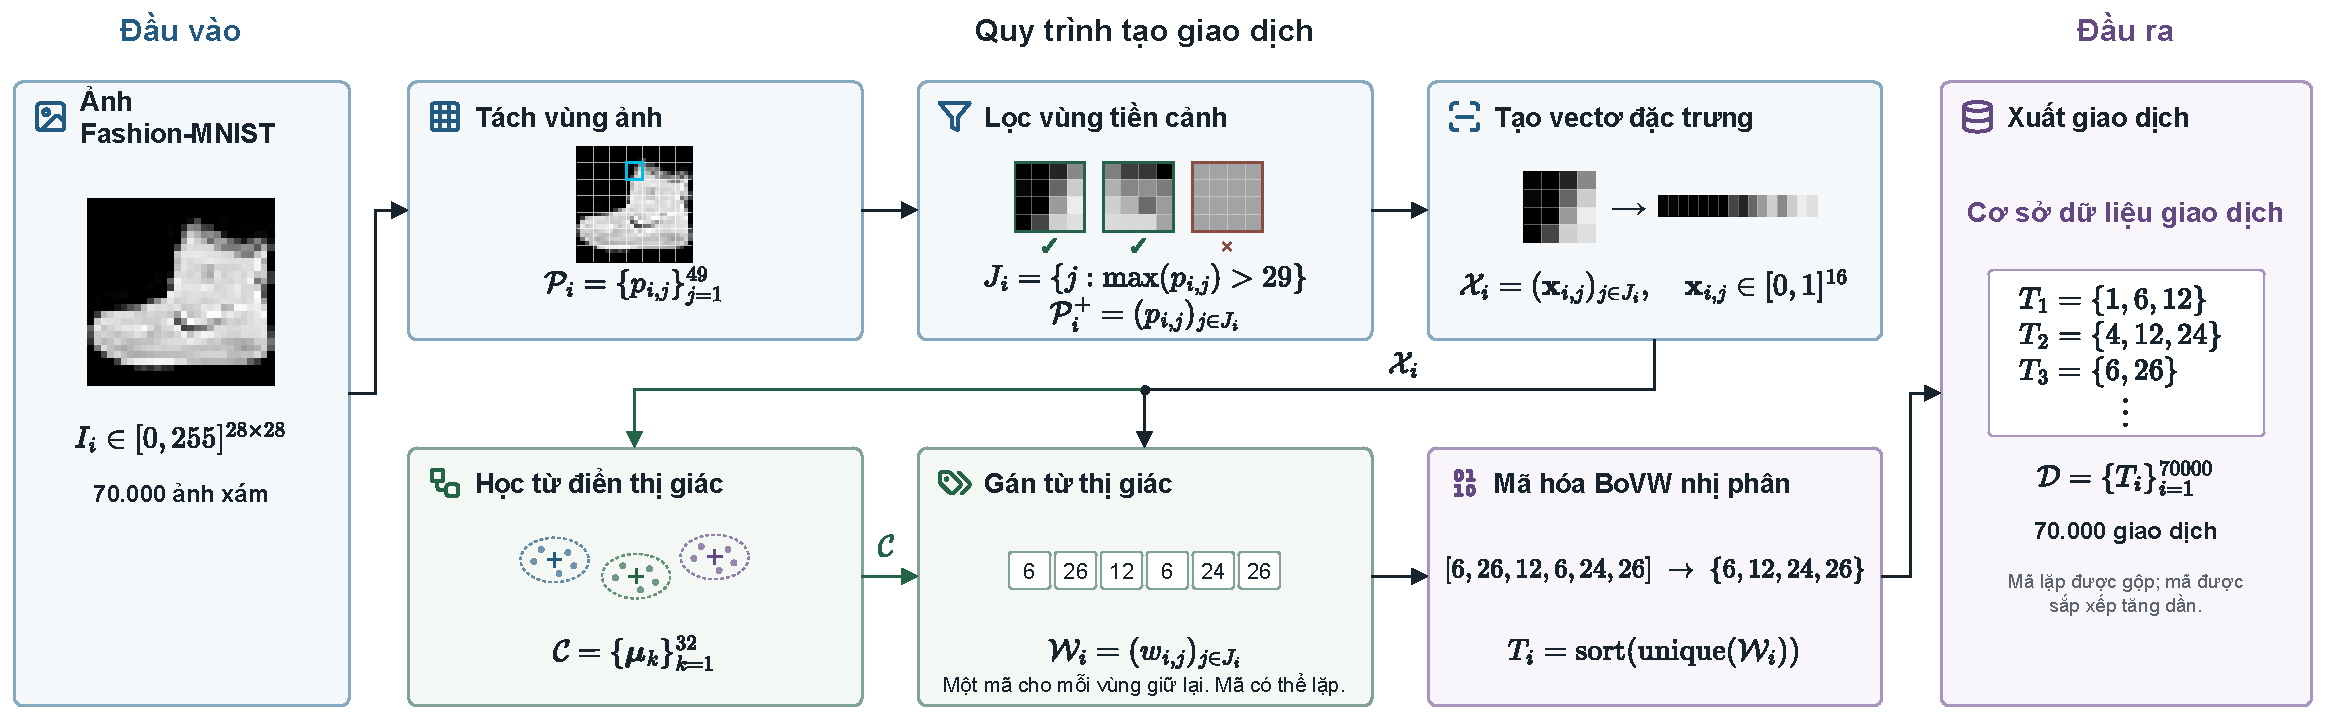
\includegraphics[width=\textwidth]{figures/diagram/TC_pipeline.pdf}
    \caption{Quy trình tạo giao dịch từ ảnh Fashion-MNIST. Nhóm học một từ điển chung từ các vùng giữ lại trên toàn bộ 70.000 ảnh rồi dùng từ điển đó để gán mã cho từng vùng. Các mã và giao dịch trong hình dùng để minh họa.}
    \label{fig:fashion_tc_pipeline}
\end{figure*}

Nhóm dùng túi từ thị giác (\textit{bag of visual words}, BoVW)~\cite{Sivic03}
để biểu diễn mỗi ảnh bằng các vùng ảnh nhỏ (\textit{patch}).
Trong khảo sát tiền xử lý, ở mức loại khoảng 39,3\% số vùng,
vùng kích thước $4\times4$ pixel làm mất 5,92\% tổng độ lớn gradient,
so với 14,00\% khi dùng vùng $7\times7$ pixel. Nhóm chọn kích thước
$4\times4$ pixel để giữ được nhiều biến thiên mức xám cục bộ hơn.

Mỗi ảnh $28\times28$ pixel được chia thành lưới $7\times7$ gồm
49 vùng không chồng lấn, mỗi vùng có kích thước $4\times4$ pixel.
Nhóm giữ vùng có ít nhất một pixel với mức xám lớn hơn 29. Giá trị 29 là phân vị
thứ 10 của các pixel khác 0. Quy tắc này loại 37,50\% số vùng,
làm mất 4,41\% tổng độ lớn gradient và vẫn giữ được vùng ảnh ở
cả 70.000 ảnh. Mỗi vùng được biểu diễn bằng vectơ đặc trưng
(\textit{descriptor}) gồm 16 giá trị mức xám, chuẩn hóa về $[0,1]$.

K-means~\cite{lloyd} gom các vectơ thành 32 cụm. Các tâm cụm
$\mathcal{C}=\{\boldsymbol{\mu}_k\}_{k=1}^{32}$ tạo thành từ điển
thị giác. Mỗi vectơ $\mathbf{x}_{i,j}$ của vùng $j$ trong ảnh $i$
nhận mã của tâm gần nhất
\begin{equation}
 w_{i,j}=\arg\min_{1\leq k\leq32}
          \|\mathbf{x}_{i,j}-\boldsymbol{\mu}_k\|_2^2.
\end{equation}
Bảng~\ref{tab:kmeans_configuration} trình bày cấu hình đã dùng.
Kết quả khảo sát số cụm được trình bày ở Phụ lục~\ref{sec:fashion-reproduction}.

\begin{table}[!t]
    \centering
        \caption{Cấu hình K-means trong thí nghiệm Fashion-MNIST}
    \label{tab:kmeans_configuration}
    \footnotesize
    \setlength{\tabcolsep}{3pt}
    \begin{tabular}{@{}p{0.40\columnwidth} p{0.55\columnwidth}@{}}
        \hline
        \textbf{Tham số} & \textbf{Giá trị} \\
        \hline
        Phương pháp & K-means toàn bộ, khởi tạo K-means++~\cite{kmpp} \\
        Dữ liệu phân cụm & 2.143.746 vectơ từ 70.000 ảnh \\
        Vectơ đặc trưng & 16 giá trị pixel xám đã chuẩn hóa \\
        Số cụm ($K$), seed & 32, 123 \\
        Giới hạn lặp, dung sai & 400, $10^{-4}$ \\
        \hline
    \end{tabular}
\end{table}

Với ảnh $I_i$, gọi $J_i$ là tập chỉ số các vùng được giữ lại và
$\mathcal{W}_i=(w_{i,j})_{j\in J_i}$ là dãy mã của các vùng đó.
BoVW nhị phân tạo giao dịch
$T_i=\operatorname{sort}(\operatorname{unique}(\mathcal{W}_i))$.
Mỗi mã được ghi một lần và các mã được sắp tăng dần. Tọa độ vùng
được lưu riêng để truy vết. Sau bước này, cả 70.000 giao dịch đều
có ít nhất một mã, với độ dài trung bình khoảng 12,23 mã.

Khảo sát năm kích thước từ điển với ba seed chọn $K=32$ làm cấu hình
cơ sở: ở ngưỡng hỗ trợ 3\%, số cặp phổ biến trung bình là 487,3,
so với 120 tại $K=16$ và 1.451,3 tại $K=64$; độ dài giao dịch trung
bình tại $K=32$ là 12,26 mã, thấp hơn mức 15,04 mã tại $K=64$.
BoVW nhị phân được giữ làm biểu diễn chính vì mỗi giao dịch chỉ ghi
nhận các mã khác nhau cùng xuất hiện, không gắn chúng với vị trí cố
định. Các biểu diễn theo vùng và dải được dùng để đối chiếu ảnh hưởng
của vị trí. Độ méo tiếp tục giảm khi tăng $K$, nên $K=32$ là lựa chọn
thực dụng theo độ gọn và khối lượng mẫu cần rà soát, không phải mức
tối ưu đã được chứng minh. Bảng khảo sát nhiều seed được trình bày ở
Phụ lục~\ref{sec:fashion-reproduction}.

\subsubsection{Thiết kế thực nghiệm khai thác}
Nhóm dùng Eclat với Set và BitVector trên cùng bộ giao dịch BoVW
nhị phân, ở sáu ngưỡng hỗ trợ từ 80\% đến 5\%. Dải ngưỡng cho
phép quan sát từ những tổ hợp có mặt trong phần lớn ảnh đến
những tổ hợp ít gặp hơn nhưng vẫn xuất hiện trong ít nhất
3.500 ảnh. Bảng~\ref{tab:eclat_backend_comparison} ghi số hỗ trợ
tối thiểu tương ứng với từng ngưỡng.

Với mỗi ngưỡng, nhóm đối chiếu từng tập mục và số hỗ trợ giữa
hai phiên bản. Thời gian được đo trong tiến trình Julia riêng.
Mỗi cấu hình được đo một lần, từ đọc giao dịch đến ghi kết quả,
không có lượt làm nóng.

\subsubsection{Kết quả K-means và khai thác tập mục phổ biến}
\label{subsec:fashion_fim_results}

K-means hội tụ sau 220 vòng và mất 137,47 giây. Cả 32 cụm đều
có vectơ được gán, với 11,75\% số vectơ thuộc cụm lớn nhất.
Khoảng cách bình phương trung bình từ vectơ đến tâm được gán
là 0,351112. Entropy chuẩn hóa đạt 0,9265 trên thang từ 0 đến 1,
cho thấy các vectơ được phân bố qua nhiều cụm.

Hai phiên bản trả về cùng các tập mục và cùng số hỗ trợ ở cả
sáu ngưỡng. Khi hạ ngưỡng, mọi tập đã tìm được ở ngưỡng cao hơn
đều vẫn xuất hiện trong kết quả (Bảng~\ref{tab:eclat_backend_comparison}).

\begin{table}[!t]
    \centering
    \caption{Số tập mục phổ biến theo ngưỡng hỗ trợ}
    \label{tab:eclat_backend_comparison}
    \footnotesize
    \setlength{\tabcolsep}{4pt}
    \begin{tabular}{@{}c r r r c@{}}
        \toprule
        \textbf{Ngưỡng} & \textbf{Số hỗ trợ tối thiểu} &
        \textbf{Set} & \textbf{BitVector} & \textbf{Giống nhau} \\
        \midrule
        80\% & 56.000 & 0 & 0 & Có \\
        60\% & 42.000 & 1 & 1 & Có \\
        40\% & 28.000 & 11 & 11 & Có \\
        20\% & 14.000 & 145 & 145 & Có \\
        10\% & 7.000 & 1.098 & 1.098 & Có \\
         5\% & 3.500 & 6.185 & 6.185 & Có \\
        \bottomrule
    \end{tabular}
\end{table}

Ở ngưỡng 5\%, Eclat tìm được 6.185 tập phổ biến, trong đó các
tập có ba hoặc bốn mã chiếm 83,25\%. Phụ lục~\ref{sec:fashion-reproduction}
trình bày phân bố theo độ dài. Ở ngưỡng này, Set mất 20,94 giây
và BitVector mất 8,73 giây. Tại 40\%, Set lại nhanh hơn một chút
(Hình~\ref{fig:eclat_performance}). Các chênh lệch chỉ mô tả
một lượt chạy ở mỗi ngưỡng.

\begin{figure}[!t]
    \centering
    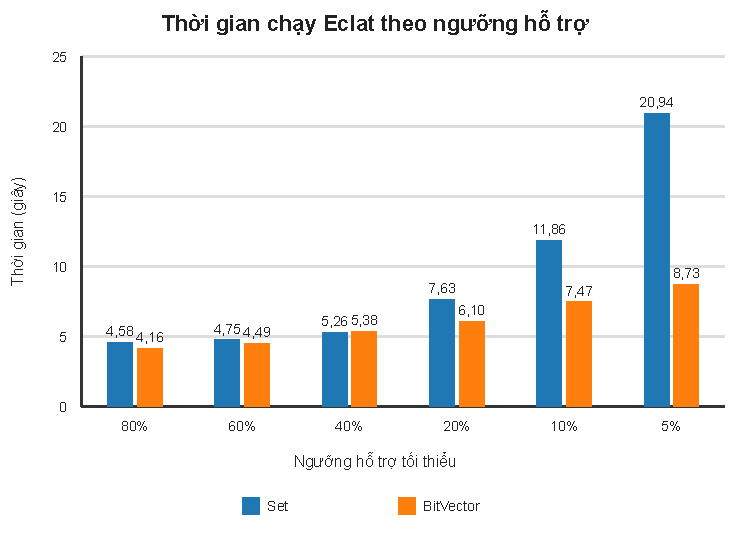
\includegraphics[width=\columnwidth]{figures/notebook3/eclat_performance.pdf}
    \caption{Thời gian chạy một lượt theo ngưỡng hỗ trợ. Nhãn TID-set (Set) chỉ phiên bản dùng cấu trúc Set.}
    \label{fig:eclat_performance}
\end{figure}

\subsubsection{Truy vết một mẫu thị giác}
\label{subsec:visual_pattern_interpretation}

Mẫu $\{6,12\}$ là tập nhiều mã có độ hỗ trợ cao nhất trong
kết quả ở ngưỡng 5\%. Mẫu có mặt trong 29.223 ảnh, tương ứng
41,75\% toàn bộ dữ liệu. Phép đếm trực tiếp trên các giao dịch
cho cùng kết quả với Eclat.

Hình~\ref{fig:current_pattern_6_12} cho thấy hai vùng được
gán mã 6 và 12 trong một ảnh, bên cạnh hai tâm cụm tương ứng.
BoVW nhị phân ghi nhận sự có mặt của hai mã ở bất kỳ vị trí nào.
Các mã 6 và 12 được xác định theo từ điển của thí nghiệm.

\begin{figure*}[!tbp]
    \centering
    \begin{tabular}{ccccc}
        
\includegraphics[width=0.17\textwidth]{figures/current_pattern/supporting_image.png} &
        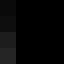
\includegraphics[width=0.17\textwidth]{figures/current_pattern/word_6_actual.png} &
        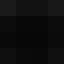
\includegraphics[width=0.17\textwidth]{figures/current_pattern/word_6_centroid.png} &
        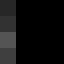
\includegraphics[width=0.17\textwidth]{figures/current_pattern/word_12_actual.png} &
        
\includegraphics[width=0.17\textwidth]{figures/current_pattern/word_12_centroid.png} \\
        Ảnh minh họa & Vùng mã 6 & Tâm mã 6 & Vùng mã 12 & Tâm mã 12
    \end{tabular}
    \caption{Ảnh và các vùng được truy vết cho mẫu $\{6,12\}$. Hai tâm cụm là các vectơ mức xám hiển thị dưới dạng vùng $4\times4$.}
    \label{fig:current_pattern_6_12}
\end{figure*}

\subsubsection{Phân bố mẫu theo lớp}
\label{subsec:fim_class_applications}

Gọi $P(X)$ là tỷ lệ ảnh chứa mẫu $X$ trên toàn bộ dữ liệu và
$P(X\mid c)$ là tỷ lệ ảnh chứa mẫu trong lớp $c$. Hai tỷ lệ này
cho phép tính hệ số làm giàu (\textit{enrichment})
\begin{equation}
    E(X,c)=\frac{P(X\mid c)}{P(X)}.
    \label{eq:fim_F_class_enrichment}
\end{equation}
Giá trị lớn hơn 1 cho biết tỷ lệ ảnh chứa mẫu trong lớp cao hơn tỷ lệ trên toàn bộ ảnh. Bảng~\ref{tab:pattern_class_distribution} ghi kết quả cho mẫu $\{6,12\}$.

\begin{table}[!t]
    \centering
    \caption{Phân bố mẫu $\{6,12\}$ theo lớp}
    \label{tab:pattern_class_distribution}
    \scriptsize
    \setlength{\tabcolsep}{2pt}
    \begin{tabular}{@{}l r r r@{}}
        \toprule
        \textbf{Lớp} & \textbf{Ảnh chứa mẫu} & \textbf{Tỷ lệ trong lớp} & \textbf{Hệ số làm giàu} \\
        \midrule
        T-shirt/top & 4.354 & 62,20\% & 1,490 \\
        Trouser & 1.263 & 18,04\% & 0,432 \\
        Pullover & 3.528 & 50,40\% & 1,207 \\
        Dress & 3.144 & 44,91\% & 1,076 \\
        Coat & 3.593 & 51,33\% & 1,230 \\
        Sandal & 3.360 & 48,00\% & 1,150 \\
        Shirt & 4.323 & 61,76\% & 1,479 \\
        Sneaker & 1.383 & 19,76\% & 0,473 \\
        Bag & 2.927 & 41,81\% & 1,002 \\
        Ankle boot & 1.348 & 19,26\% & 0,461 \\
        \bottomrule
    \end{tabular}
\end{table}

Mẫu xuất hiện ở cả mười lớp. Tỷ lệ dao động từ 18,04\% ở Trouser đến 62,20\% ở T-shirt/top. Chênh lệch này cho thấy cùng một mẫu có thể phổ biến hơn ở một số lớp dù xuất hiện rộng trong toàn bộ dữ liệu.

Nhãn lớp chỉ được dùng sau bước khai thác để tính các tỷ lệ.
Vì từ điển thị giác và các tập mục đều được xây dựng từ cả hai
tập ảnh gốc, các tỷ lệ này mô tả chính bộ dữ liệu đã khai thác.

\subsubsection{Mức độ làm giàu theo ngưỡng hỗ trợ}

Với mỗi tập mục $X$, đặt $E_{\max}(X)=\max_c E(X,c)$, tức hệ số làm giàu lớn nhất trong mười lớp. Bảng~\ref{tab:fashion_enrichment_thresholds} cho thấy cả trung vị $E_{\max}$ lẫn tỷ lệ tập mục có $E_{\max}\geq2$ tăng khi hạ ngưỡng hỗ trợ. Tại 5\%, 4.180 trong 6.185 tập mục (67,58\%) xuất hiện trong ít nhất một lớp với tỷ lệ gấp đôi tỷ lệ chung trở lên. Ở các ngưỡng từ 40\%, không có tập nào đạt mức này. Mức làm giàu còn phụ thuộc vào độ phổ biến chung của mẫu. Ví dụ, mẫu đã có mặt trong 60\% toàn bộ ảnh chỉ có thể đạt hệ số tối đa khoảng 1,67, kể cả khi xuất hiện trong mọi ảnh của một lớp.

\begin{table}[!t]
    \centering
    \caption{Hệ số làm giàu lớn nhất theo ngưỡng hỗ trợ}
    \label{tab:fashion_enrichment_thresholds}
    \scriptsize
    \setlength{\tabcolsep}{3pt}
    \begin{tabular}{@{}c r r r r@{}}
        \toprule
        \textbf{Ngưỡng} & \textbf{Số tập mục} & \textbf{Trung vị $E_{\max}$} &
        \textbf{$E_{\max}\geq2$} & \textbf{Tỷ lệ} \\
        \midrule
        80\% & 0 & -- & 0 & -- \\
        60\% & 1 & 1,294 & 0 & 0\% \\
        40\% & 11 & 1,490 & 0 & 0\% \\
        20\% & 145 & 1,735 & 26 & 17,93\% \\
        10\% & 1.098 & 1,998 & 543 & 49,45\% \\
         5\% & 6.185 & 2,225 & 4.180 & 67,58\% \\
        \bottomrule
    \end{tabular}
\end{table}

Hình~\ref{fig:fashion_enrichment_summary} cho thấy phân bố hệ số lớn nhất theo ngưỡng và số mẫu có hệ số từ 2 trở lên ở từng lớp. Trong khi biểu đồ (b) đếm mẫu riêng theo lớp, $E_{\max}$ chỉ lấy lớp có tỷ lệ tương đối cao nhất để mô tả mức tập trung của từng mẫu.

\begin{figure*}[!tbp]
    \centering
    \begin{minipage}[t]{0.48\textwidth}
        \centering
        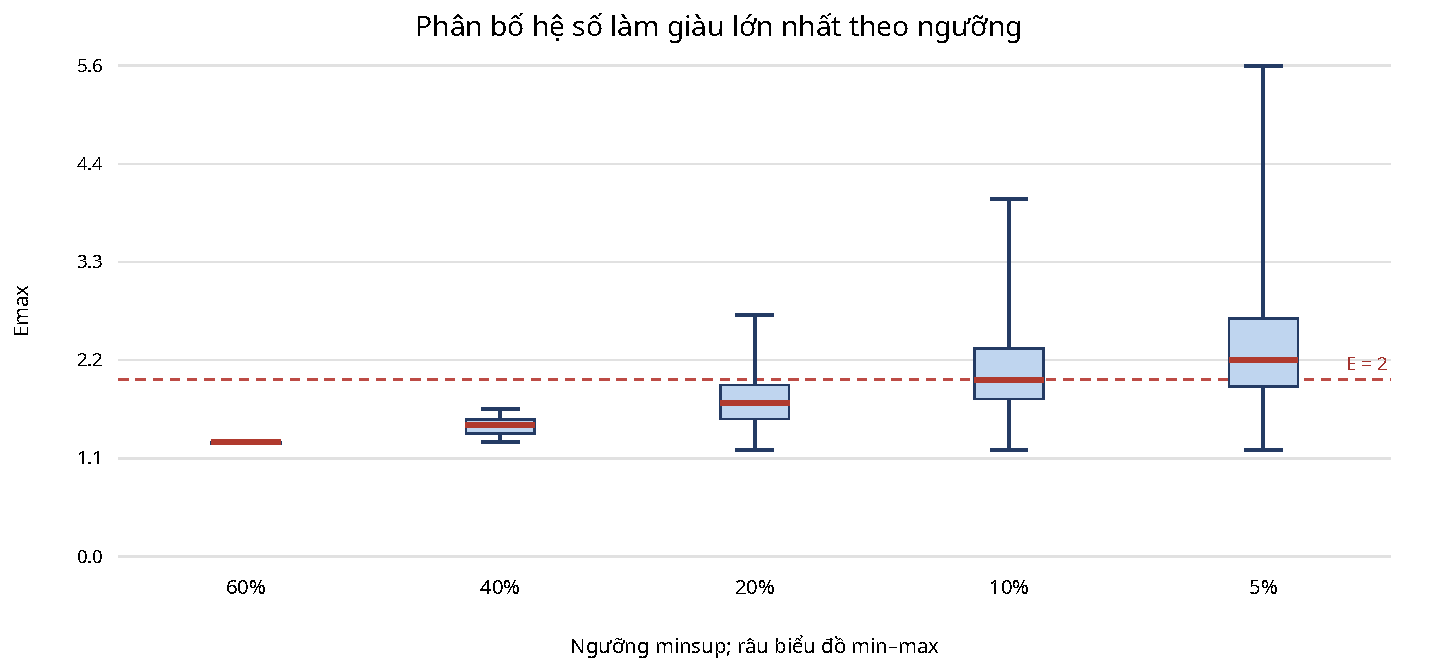
\includegraphics[width=\linewidth]{figures/notebook3/enrichment_by_threshold.pdf}
        \\
        \small (a) Phân bố $E_{\max}$ theo ngưỡng hỗ trợ.
    \end{minipage}\hfill
    \begin{minipage}[t]{0.48\textwidth}
        \centering
        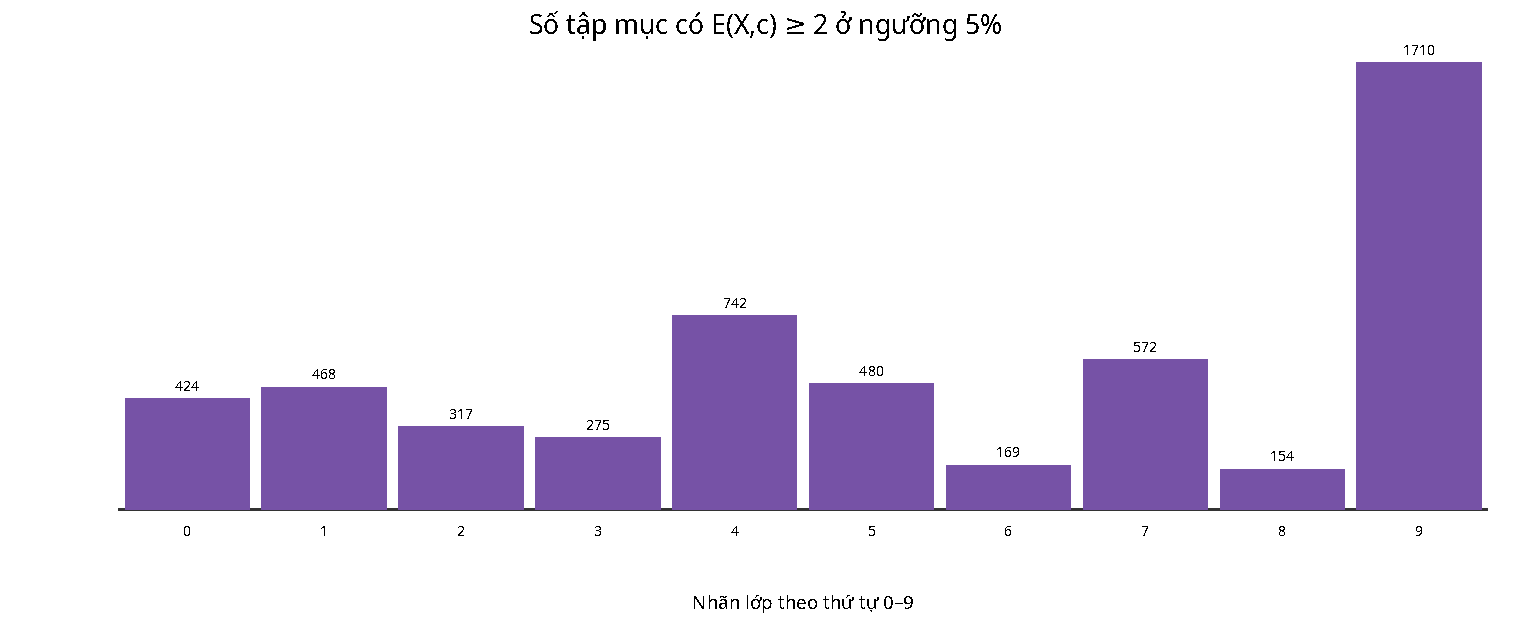
\includegraphics[width=\linewidth]{figures/notebook3/patterns_enriched_by_class.pdf}
        \\
        \small (b) Số tập mục có $E(X,c)\geq2$ theo lớp.
    \end{minipage}
    \caption{Mức độ làm giàu của các tập mục khai thác được. Các thanh dọc ở biểu đồ (a) biểu thị khoảng giá trị nhỏ nhất đến lớn nhất. Biểu đồ (b) đếm riêng theo từng lớp, nên một tập mục có thể xuất hiện trong nhiều cột.}
    \label{fig:fashion_enrichment_summary}
\end{figure*}

\subsubsection{Các mẫu nhiều mã nổi bật trong từng lớp}

Để xem tổ hợp từ thị giác nào gắn với từng lớp, nhóm chọn cho mỗi lớp một tập nhiều mã có $E(X,c)$ cao nhất trong số các tập mà ít nhất 10\% ảnh của lớp chứa tập đó. Hình~\ref{fig:fashion_class_pattern_heatmap} biểu diễn tỷ lệ chứa từng mẫu trên cả mười lớp. Ví dụ, mẫu $\{13,14,26,29\}$ có mặt trong 31,11\% ảnh Trouser và hệ số làm giàu 5,553; mẫu $\{3,10,15,22\}$ có mặt trong 25,91\% ảnh Ankle boot và hệ số 5,156.

\begin{figure*}[!tbp]
    \centering
    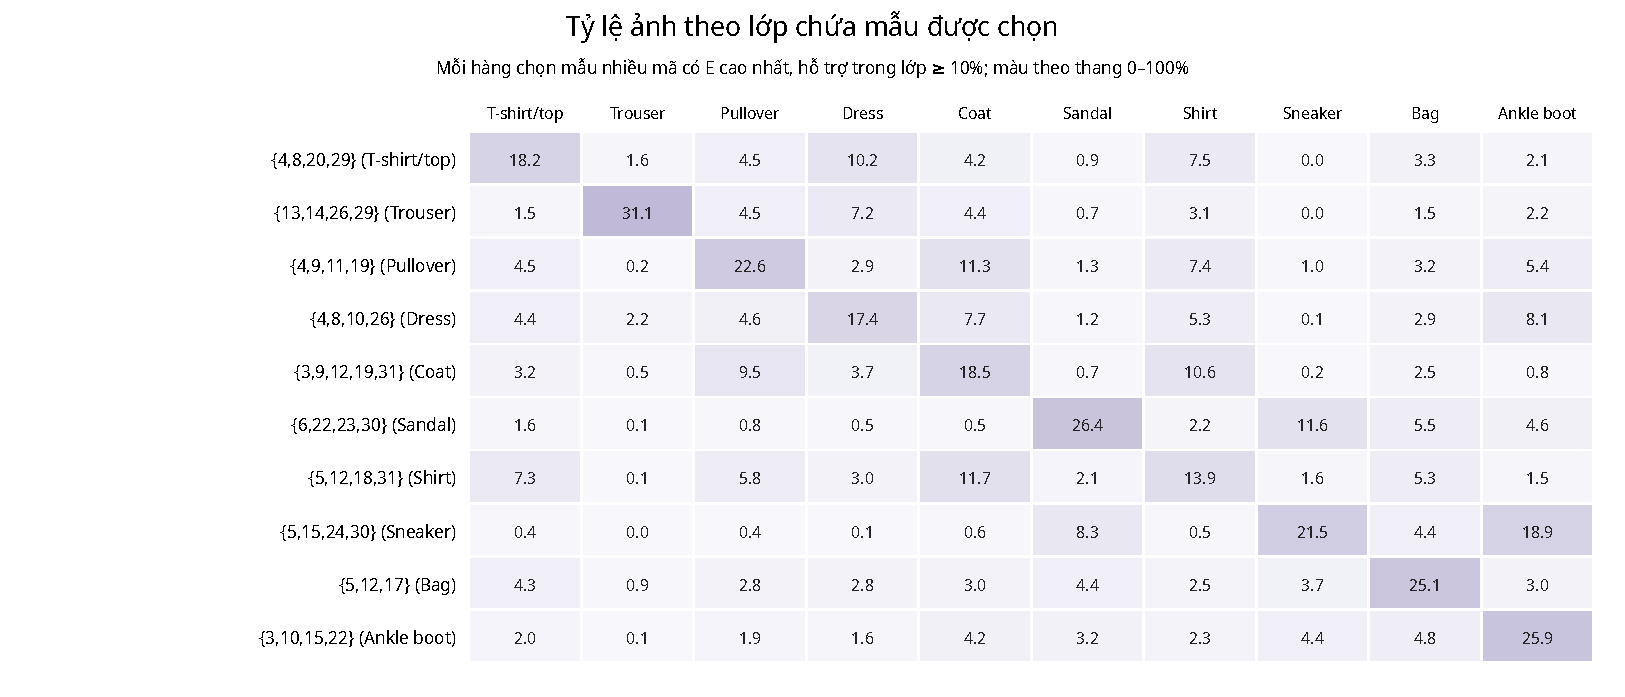
\includegraphics[width=0.98\textwidth]{figures/notebook3/class_pattern_heatmap.pdf}
    \caption{Tỷ lệ ảnh trong mỗi lớp chứa mẫu nhiều mã được chọn cho hàng đó. Mẫu của từng hàng được chọn theo hệ số làm giàu cao nhất, với điều kiện tỷ lệ hỗ trợ trong lớp đạt ít nhất 10\%.}
    \label{fig:fashion_class_pattern_heatmap}
\end{figure*}

Các ô ngoài đường chéo cho thấy mẫu được chọn ở một lớp cũng có thể xuất hiện ở lớp khác. Hình vì vậy giúp xác định mẫu nào đáng khảo sát tiếp. Giá trị dự đoán cần được đánh giá trên dữ liệu độc lập với bước chọn mẫu.

\subsubsection{Hướng ứng dụng và phát triển các mô hình khác}

Các tập mục thường gặp hơn ở một lớp là những đặc trưng ứng viên
cho mô hình phân loại. Có thể dùng các mẫu này để giải thích ảnh
chứa tổ hợp mã nào hoặc để truy vấn những ảnh có chung tổ hợp.

Với $m$ tập mục đã chọn $P_1,\ldots,P_m$, vectơ đặc trưng của ảnh $I_i$ là $\boldsymbol{\phi}(I_i)=(\phi_1(I_i),\ldots,\phi_m(I_i))$. Mỗi thành phần cho biết giao dịch $T_i$ có chứa tập mục tương ứng hay không:
\begin{equation}
    \phi_j(I_i)=\mathbf{1}\!\left[P_j\subseteq T_i\right],
    \qquad j=1,\ldots,m.
    \label{eq:fim_pattern_features}
\end{equation}
Nhóm có thể so sánh ba biểu diễn trên cùng cách chia dữ liệu:
BoVW nhị phân, vectơ chỉ báo tập mục và biểu diễn có xét vị trí.
Với mỗi biểu diễn, dùng cùng nhóm bộ phân loại, chẳng hạn hồi quy
logistic, SVM tuyến tính và cây quyết định. So sánh các giá trị của
số cụm, ngưỡng hỗ trợ, cấu hình không gian và tham số mô hình
theo cùng quy trình chọn tham số.

Đề xuất dùng kiểm định chéo phân tầng năm phần
(\textit{stratified five-fold cross-validation}) trên 60.000 ảnh
huấn luyện. Mỗi lượt học lại từ điển, khai thác và chọn mẫu, rồi
huấn luyện mô hình chỉ trên bốn phần. Phần còn lại dùng để đánh
giá cấu hình. Có thể báo cáo trung bình và độ lệch chuẩn của độ
chính xác và F1 vĩ mô qua năm lượt, kèm ma trận nhầm lẫn để xem những lớp dễ bị nhầm với nhau.

Sau khi chọn cấu hình, huấn luyện lại trên toàn bộ 60.000 ảnh
và đánh giá một lần trên 10.000 ảnh kiểm thử giữ riêng. Kết quả
so với BoVW nhị phân trên tập này sẽ cho biết đặc trưng tập mục
hoặc thông tin vị trí có cải thiện khả năng dự đoán hay không.


\subsection{Tổng kết hai ứng dụng}
Hai ứng dụng dùng cùng thuật toán nhưng khác nhau ở ý nghĩa của
mỗi mục. Trong Groceries, mã mục ánh xạ trực tiếp đến tên sản phẩm,
nên có thể đọc luật theo thành phần của giỏ hàng. Trong Fashion-MNIST,
mỗi mục là mã của một nhóm vùng ảnh tương tự nhau. Việc xem lại các
vùng gốc giúp giải thích mã thị giác đang đại diện cho đặc trưng nào.
Kết quả ở cả hai ứng dụng mô tả các tổ hợp thường xuất hiện cùng
nhau trong dữ liệu quan sát. Giá trị của chúng đối với gợi ý sản phẩm
và phân loại ảnh cần được kiểm chứng trên dữ liệu mới.

\begin{thebibliography}{99}
\bibitem{zaki} M. J. Zaki, ``Scalable Algorithms for Association Mining,''
\emph{IEEE Transactions on Knowledge and Data Engineering}, vol. 12, no. 3,
pp. 372--390, 2000, doi: 10.1109/69.846291.
\bibitem{spmf} P. Fournier-Viger et al., ``The SPMF Open-Source Data Mining
Library Version 2,'' in \emph{ECML PKDD 2016}, LNCS 9853, pp. 36--40, 2016,
doi: 10.1007/978-3-319-46131-1\_8.
\bibitem{agrawal} R. Agrawal and R. Srikant, ``Fast Algorithms for Mining
Association Rules,'' in \emph{Proceedings of the 20th VLDB Conference},
pp. 487--499, 1994.
\bibitem{julia} J. Bezanson, A. Edelman, S. Karpinski, and V. B. Shah,
``Julia: A Fresh Approach to Numerical Computing,'' \emph{SIAM Review},
vol. 59, no. 1, pp. 65--98, 2017, doi: 10.1137/141000671.
\bibitem{fimi} FIMI Repository, ``Frequent Itemset Mining Dataset Repository.''
[Online]. Available: \url{https://fimi.uantwerpen.be/data/}.
\bibitem{groceries} stedy, ``Machine Learning with R datasets: groceries.csv.''
[Online]. Available: \url{https://github.com/stedy/Machine-Learning-with-R-datasets/blob/master/groceries.csv}.
\bibitem{Sivic03} J. Sivic and A. Zisserman, ``Video Google: A Text Retrieval
Approach to Object Matching in Videos,'' in \emph{Proc. ICCV}, vol. 2,
pp. 1470--1477, 2003.
\bibitem{lloyd} S. P. Lloyd, ``Least Squares Quantization in PCM,''
\emph{IEEE Transactions on Information Theory}, vol. 28, no. 2,
pp. 129--137, 1982, doi: 10.1109/TIT.1982.1056489.
\bibitem{kmpp} D. Arthur and S. Vassilvitskii, ``k-means++: The Advantages of
Careful Seeding,'' in \emph{Proc. SODA}, pp. 1027--1035, 2007.
\bibitem{Xiao2017} H. Xiao, K. Rasul, and R. Vollgraf, ``Fashion-MNIST: A
Novel Image Dataset for Benchmarking Machine Learning Algorithms,''
\emph{arXiv preprint arXiv:1708.07747}, 2017,
doi: 10.48550/arXiv.1708.07747.
\end{thebibliography}

\appendices
\section{Bổ sung về cài đặt và kiểm thử}
\label{sec:reproduction}
Gọi $E=\sum_{j=1}^{N}|t_j|$ là tổng số lần xuất hiện của các mục,
$F_1$ là số tập một mục đạt ngưỡng và $w$ là số bit mỗi từ máy.
Dựng tập định danh ban đầu tốn thời gian kỳ vọng $O(E)$ với Set
và $O(E+F_1\lceil N/w\rceil)$ với BitVector. Chi phí sắp các mã
mục lần lượt là $O(M\log M)$ và $O(F_1\log F_1)$. Bộ nhớ của
các vector ban đầu là $O(F_1N)$ bit, cộng thêm trạng thái đếm
$O(M)$ và các cấu trúc phục vụ quá trình duyệt. Nếu $F$ là số tập
phổ biến và $K$ là tổng độ dài các tập đó, phần lưu kết quả
cần $O(F+K)$ ô lưu trữ.

Phép đếm vét cạn được thực hiện trên 40 cơ sở dữ liệu nhỏ sinh với
hạt giống 20261116, ở ba ngưỡng 20\%, 50\% và 100\%. Lần kiểm thử
ngày 24/11/2026 trên Julia 1.13.3/Linux ghi nhận 569 mục kiểm tra đạt.
Cách chuẩn bị dữ liệu, định dạng đầu vào và lệnh chạy được mô tả trong
\href{https://github.com/NguyenVoTanDuy2006/DataMining-FIM-Project/blob/master/README.md}{hướng dẫn của dự án}.

\section{Cấu hình và số đo bổ sung}
\label{sec:benchmark-reproduction}
Trong bước chuẩn hóa, Chess và Mushroom giữ mã mục gốc. Retail và
T10I4D100K tăng mọi mã thêm một để loại mã 0 khỏi miền đầu vào.
Bảng~\ref{tab:grids} ghi các dải ngưỡng. Báo cáo tổng hợp 560 lượt đo
gồm 420 lượt đo thời gian toàn tiến trình, 40 lượt đo đỉnh bộ nhớ,
50 lượt theo số giao dịch và 50 lượt theo độ dài giao dịch.
\href{https://github.com/NguyenVoTanDuy2006/DataMining-FIM-Project/blob/master/docs/report_benchmark.md}{Hướng dẫn tái lập benchmark}
mô tả quy trình đo. Hồ sơ local tại \path{results/colab/benchmark_20261125/}
lưu số đo từng lượt, mã phiên bản nguồn và môi trường.

\begin{reporttable}
\caption{Dải minsup, đơn vị phần trăm; điểm thứ tư dùng cho Peak RSS.}
\label{tab:grids}
\footnotesize
\begin{tabular}{lp{0.65\columnwidth}}\toprule
CSDL & Bảy ngưỡng từ cao xuống thấp\\\midrule
Chess & 95; 92,5; 90; 87,5; 85; 82,5; 80\\
Mushroom & 95; 90; 80; 70; 60; 50; 40\\
Retail & 10; 8; 6; 4; 2; 1; 0,5\\
T10I4D100K & 3; 2,5; 2; 1,5; 1; 0,75; 0,5\\\bottomrule
\end{tabular}
\end{reporttable}

Các tập con Retail được lấy từ cùng một hoán vị giao dịch, sinh
với hạt giống 20261116. Khi tạo dữ liệu tổng hợp, nhóm hoán vị danh
sách $M=64$ mục riêng cho từng giao dịch rồi lấy $L$ mục đầu.
Với cách chọn đều này, xác suất $p_2$ để một cặp cụ thể có mặt là
\begin{equation}
 p_2=\frac{L(L-1)}{M(M-1)}.
\end{equation}
Trong $N=5.000$ giao dịch, số hỗ trợ kỳ vọng $Np_2$ lần lượt
khoảng 164 và 298 khi $L=12$ và $L=16$. Hai giá trị nằm hai
phía ngưỡng 250, phù hợp với bước tăng số kết quả quan sát được.

\subsection{Số đo Groceries theo công đoạn}
Bảng~\ref{tab:groceries-timing} ghi số đo theo từng công đoạn.
Thời gian toàn quy trình bao gồm đọc dữ liệu, chuẩn hóa, mã hóa,
khai thác và sinh luật trong tiến trình đã nạp mã. Các công đoạn
được đo độc lập nên trung vị của chúng không cộng thành trung vị
của toàn quy trình. Tổng cộng 140 mẫu và cấu hình được lưu local tại
\path{results/colab/groceries_20261125/}.
Xem \href{https://github.com/NguyenVoTanDuy2006/DataMining-FIM-Project/blob/master/docs/report_groceries.md}{hướng dẫn tái lập Groceries}.

\begin{reporttable}
\caption{Số đo Groceries ở ngưỡng hỗ trợ 1\% và độ tin cậy 50\%. Đơn vị ms, năm lượt sau làm nóng.}
\label{tab:groceries-timing}
\centering\footnotesize
\begin{tabular}{lrrr}\toprule
Phạm vi & Trung vị & Nhỏ nhất & Lớn nhất\\\midrule
Khai thác & 55,05 & 50,33 & 92,56\\
Sinh luật & 1,24 & 1,21 & 1,37\\
Toàn quy trình & 82,62 & 76,67 & 88,63\\\bottomrule
\end{tabular}
\end{reporttable}

\section{Số liệu bổ sung cho Fashion-MNIST}
\label{sec:fashion-reproduction}
Bảng~\ref{tab:fashion-lengths} trình bày phân bố độ dài ở ngưỡng
hỗ trợ 5\%. Bộ giao dịch có tổng cộng 856.373 lượt xuất hiện mã
và độ dài trung vị là 12 mã.

\begin{reporttable}
\caption{Số tập phổ biến theo độ dài ở ngưỡng hỗ trợ 5\%.}
\label{tab:fashion-lengths}
\small
\begin{tabular}{lrrrrrr}\toprule
Số mã & 1 & 2 & 3 & 4 & 5 & 6 \\\midrule
Số tập & 32 & 482 & 2.468 & 2.681 & 508 & 14 \\\bottomrule
\end{tabular}
\end{reporttable}

Ví dụ truy vết trong phần chính được chọn theo độ hỗ trợ. Xem
\href{https://github.com/NguyenVoTanDuy2006/DataMining-FIM-Project/blob/master/docs/UD2/TC_plan.md}{khảo sát tiền xử lý ảnh}
để đối chiếu lựa chọn kích thước vùng và ngưỡng lọc nền.

Khảo sát gồm năm kích thước từ điển, mỗi kích thước chạy với ba
seed. Cả 15 lượt K-means đều hội tụ và sử dụng đủ số cụm. Bảng
~\ref{tab:fashion-k-selection} tổng hợp độ méo, độ dài giao dịch
BoVW nhị phân và số cặp phổ biến trung bình tại ngưỡng hỗ trợ 3\%
với giới hạn độ dài hai.

\begin{reporttable}
\caption{Kết quả khảo sát K-means và giao dịch theo kích thước từ điển.}
\label{tab:fashion-k-selection}
\scriptsize
\setlength{\tabcolsep}{3pt}
\begin{tabular}{crrr}\toprule
$K$ & $\bar{D}\pm s_D$ & $\overline{|T|}$ & Số cặp phổ biến \\
\midrule
16  & $0{,}4463\pm0{,}0065$ & 8,82  & 120,0 \\
32  & $0{,}3488\pm0{,}0037$ & 12,26 & 487,3 \\
64  & $0{,}2720\pm0{,}0006$ & 15,04 & 1.451,3 \\
128 & $0{,}2179\pm0{,}0005$ & 17,92 & 1.489,7 \\
256 & $0{,}1769\pm0{,}0001$ & 20,37 & 638,3 \\
\bottomrule
\end{tabular}
\end{reporttable}

Độ méo giảm theo $K$, nhưng không có điểm gãy rõ tại 32. Lựa chọn
$K=32$ cân bằng giữa giao dịch gọn và số cặp đủ lớn để phân tích:
giao dịch trung bình ngắn hơn tại $K=64$, trong khi số cặp phổ biến
nhiều hơn rõ rệt tại $K=16$. Số đếm này phản ánh khối lượng mẫu cần
rà soát, không đo trực tiếp chất lượng ngữ nghĩa. BoVW nhị phân được
giữ làm biểu diễn chính vì nó ghi nhận đồng xuất hiện mà không áp đặt
vị trí; biểu diễn theo vùng và dải dùng để đối chiếu tác động của
thông tin vị trí. Các kết quả này hỗ trợ một lựa chọn thực dụng cho
phân tích khai phá mẫu, không chứng minh cấu hình tối ưu hay giá trị
dự đoán.
\end{document}
